%%%% Semesterprojekt rapport gruppe 2 %%%%
%%%% Elektronik Q1/Q2 2016 %%%%

% Kan anvendes til journaler eller afleveringer
\documentclass[11pt, a4paper, twoside, openany]{memoir}

\usepackage[utf8]{inputenc}		% Dansk input encoding (tegn)
\usepackage[danish]{babel}		% Danske formuleringer / orddeling
\usepackage[T1]{fontenc}		% Output-indkodning af tegnsaet (T1)


%%% Memoir indstillinger
%% Afstand mellem afsnit og videre
%% NIX PILLE - medmindre strengt nødvendigt
\setaftersubsubsecskip{6pt}	
\setbeforesubsubsecskip{6pt}
%\setaftersubsecskip{6pt}
%\setbeforesubsecskip{-\baselineskip}
%\setaftersecskip{6pt}
%\setbeforesecskip{-\baselineskip}
%\setaftersecskip{1ex}

\raggedbottom



\chapterstyle{section}
\usepackage{url}

% ¤¤ Marginer ¤¤ %
\setlrmarginsandblock{3.5cm}{2.5cm}{*}		% \setlrmarginsandblock{Indbinding}{Kant}{Ratio}
\setulmarginsandblock{3.0cm}{2.5cm}{*}		% \setulmarginsandblock{Top}{Bund}{Ratio}
\checkandfixthelayout

%%% Font valg %%%
\usepackage{mathpazo}	%Palatinofont - matematikformler
\usepackage{eulervm}		%Palatinofont

%%% FIGURER OG TABELLER %%%
\usepackage{graphicx} 						% Haandtering af eksterne billeder (JPG, PNG, PDF)

\usepackage[export]{adjustbox}

\usepackage{multirow}                		% Fletning af raekker og kolonner (\multicolumn og \multirow)
\usepackage{colortbl} 						% Farver i tabeller (fx \columncolor, \rowcolor og \cellcolor)
\usepackage[dvipsnames]{xcolor}				% Definer farver med \definecolor. Se mere: http://en.wikibooks.org/wiki/LaTeX/Colors
%\usepackage{flafter}						% Soerger for at floats ikke optraeder i teksten foer deres erence
\usepackage{float}							% Muliggoer eksakt placering af floats, f.eks. \begin{figure}[H]
\usepackage{multicol}         	        	% Muliggoer tekst i spalter
%\usepackage{rotating}						% Rotation af tekst med \begin{sideways}...\end{sideways}
\usepackage{booktabs}
\usepackage{bigstrut}	% Excel2latex måskeh
\usepackage{tabularx}
\usepackage{subfig}

%%% ¤¤ Matematik mm. %%%
\usepackage{amsmath,amssymb,stmaryrd} 		% Avancerede matematik-udvidelser
\usepackage{mathtools}						% Andre matematik- og tegnudvidelser
\usepackage{textcomp}                 		% Symbol-udvidelser (f.eks. promille-tegn med \textperthousand )
\usepackage{siunitx}						% Flot og konsistent praesentation af tal og enheder med \si{enhed} og \SI{tal}{enhed}
\sisetup{output-decimal-marker = {,}}		% Opsaetning af \SI (DE for komma som decimalseparator) 
\sisetup{exponent-product=\cdot, output-product=\cdot}	%Eksponent er gange tegn, output produkt er gange tegn
\sisetup{digitsep = none}					%Almindeligt komma - ingen mellemrum aka. til eurokomma

%%% REFERENCER %%%


%%% MISC %%%
\usepackage{listings}						% Placer kildekode i dokumentet med \begin{lstlisting}...\end{lstlisting}
\definecolor{bg}{HTML}{F0F0F0}
\lstset{language=C++,
				showstringspaces = false,
				backgroundcolor = \color{bg},
                basicstyle=\ttfamily,
                keywordstyle=\color{blue}\ttfamily,
                stringstyle=\color{red}\ttfamily,
                commentstyle=\color{green}\ttfamily,
                morecomment=[l][\color{magenta}]{\#},
                extendedchars=true,
                numbers=left, numberstyle=\tiny,		% Linjenumre
                columns=flexible,						% Kolonnejustering
                breaklines, breakatwhitespace=true,		% Bryd lange linjer
                literate=%
                {æ}{{\ae}}1
                {å}{{\aa}}1
                {ø}{{\o}}1
                {Æ}{{\AE}}1
                {Å}{{\AA}}1
                {Ø}{{\O}}1
}


\usepackage{lipsum}							% Dummy text \lipsum[..]
\usepackage[shortlabels]{enumitem}			% Muliggoer enkelt konfiguration af lister
\usepackage{pdfpages}						% Goer det muligt at inkludere pdf-dokumenter med kommandoen \includepdf[pages={x-y}]{fil.pdf}	
\pdfoptionpdfminorversion=6					% Muliggoer inkludering af pdf dokumenter, af version 1.6 og hoejere

%	¤¤ Afsnitsformatering ¤¤ %
%\setlength{\parindent}{0mm}           		% Stoerrelse af indryk
\setlength{\parskip}{1.5mm}          		% Afstand mellem afsnit ved brug af double Enter
\linespread{1,1}							% Linie afstand

\usepackage{tikz}


% ¤¤ Visuelle  ¤¤ %
\usepackage[colorlinks]{hyperref}			% Danner klikbare referencer (hyperlinks) i dokumentet.
\hypersetup{colorlinks = true,				% Opsaetning af farvede hyperlinks (interne links, citeringer og URL)
	linkcolor = black,
	citecolor = black,
	urlcolor = black
}



%%% Referencer / Bibliografi %%%
\usepackage[backend=biber, sorting=none, style=numeric]{biblatex}
\bibliography{../referencer.bib}


\usepackage[draft, danish]{fixme}
\fxsetup{layout=footnote}

\graphicspath{{../fig/}{../fig}{./}}


\usepackage{rotating}
\usepackage{titlesec}

\setcounter{secnumdepth}{4}

\titleformat{\paragraph}
{\normalfont\normalsize\bfseries}{\theparagraph}{1em}{}
\titlespacing*{\paragraph}
{0pt}{3.25ex plus 1ex minus .2ex}{1.5ex plus .2ex}


%%%% Opsætning af dokument %%%%
\newcommand{\forfatter}{Gruppe 2}
\newcommand{\fag}{INDSÆT KURSUS HER}
\newcommand{\titel}{Semesterprojekt 4 Dokumentation}
\date{}

\author{\forfatter}
\title{\titel}

\setlength{\beforechapskip}{10pt}
\setlength{\afterchapskip}{10pt}

\begin{document}
%\maketitle
\begin{titlingpage}
%\thispagestyle{title}
		
		\begin{center}
				{\huge\bfseries Projekt Universal Actuator Drive}\\
				\vspace{10pt}
				
				{\Huge\bfseries Procesbeskrivelse}\\
				
				\vspace{20pt}
				
				{Diplomingeniør Elektronik}\\
				{\large Bachelorprojekt efterår 2017}\\
				
				\vspace{10pt}
				
				Ingeniørhøjskolen Aarhus Universitet\\
				Vejleder: Arne Justesen
				\vspace{10pt}
				
				19. december 2017
				\vspace{10pt}

				\vspace{50pt}
				\begin{minipage}{0.25\linewidth}
					\centering
					\hrule
					\vspace{12pt}
					Nicolai H. Fransen\\
					Studienr. 201404672
				\end{minipage}
				\hspace{10pt}
				\begin{minipage}{0.25\linewidth}
					\centering
					\hrule
					\vspace{12pt}
					Jesper Kloster\\
					Studienr. 201404571
				\end{minipage}
				\hspace{10pt}
		\end{center}
		
		\clearpage
		
	\setcounter{tocdepth}{2}
	\tableofcontents
	\clearpage
	
	%\include{tex/indledning/indledning}
	
	\chapter{Forord}

	\chapter{Indledning}
Proces er en særdeles vigtig del af et projektforløb, og består af mange forskellige elementer. En god processtruktur kan hjælpe til at give bedre overblik over perioden og gøre alle parter enige om, hvordan rapport og produkt skal udformes. Uden elementerne i en procesbeskrivelse risikerer gruppen, at arbejde i forskellige retninger, og på den måde ikke opnå optimalt samarbejde. Ved at have en række retningslinjer skrevet ned omkring, hvordan f.eks. arbejdsfordelingen og udviklingsforløbet skal foregå, er risikoen for misforståelser mindre i løbet af perioden. En veldefineret processtruktur bliver vigtigere og vigtigere, jo flere folk der arbejder sammen. Men selv i grupper af få personer, giver det optimerede arbejdsbetingelser, når der er faste måder, at gøre tingene på.  

I denne gruppe er der lagt vægt på, at opsætte en proces, der giver det bedste fundament for en god produktudvikling. Da gruppen består af to medlemmer har der med fastlagte udviklingsforløb og arbejdsfordelinger, været mere tid til udviklingen af produktet. Der er gennemgående benyttet en iterativ udviklingsproces, da det har været nødvendigt at opnå erfaring og ny viden løbende. 

Grundet gruppestørrelsen har der ikke været fordelt procesmæssige hovedansvarsområder blandt medlemmerne. Der har istedet været en flad struktur, hvor begge medlemmer har været inde over alle delene i processen.   
	\chapter{Gruppedannelse}
Gruppen er sammensat ud fra samarbejde igennem de tidligere semestre. Vi har gennemgående haft samme kurser, og har hele vejen igennem haft et godt samarbejde. Det var derfor naturligt, at skrive bacheloren sammen. Det giver samtidig også en fordel, at der på forhånd er kendskab til hinandens styrker og svagheder.


Gruppen består af 2 medlemmer, hvilket er et bevist valg, da der på den måde er større mulighed for at forme projektet og processen efter individuelle ønsker. Der er både fordele og ulemper ved at have flere inputs. Her har det været en succes at være få, da der ikke er brugt unødig tid på at diskutere småting, men istedet have tid og overskud til, at diskutere de vigtige valg mere i dybden. Ved de tidligere 4 semesterprojekter, hvor grupperne har været omkring 8 personer, har der været meget forskellige meninger om, hvordan tingene skal gøres, hvilket sløver processen. Da vi har været i gruppe sammen i 3 af tilfældene, har det været nemt at vurdere, hvad der tidligere har fungeret. Det gør, at der hurtigt nås til enighed om den optimale måde at gøre tingene på.

	\chapter{Samarbejdskontrakt}
Der er udarbejdet en samarbejdskontrakt, som kan findes i bilagsmappen. Samarbejdskontrakten definerer dele af strukturen for gruppearbejdet såsom møder. Kontrakten er mest af alt en formalitet, da antallet af gruppemedlemmer er på 2, og derfor væsentlig færre end ved tidligere semesterprojekter. Ved større grupper er der i højere grad brug for skriftlige aftaler, da der ellers kan være medlemmer som gemmer sig, eller bliver udeladt i processen. Det er ikke det store problem i en gruppe af 2 personer. Til gengæld giver det stadig en sikkerhed og en bekræftelse af, at man har de samme forventninger til udviklingsprocessen og arbejdsmentaliteten. Det giver også mulighed for at opstille rammer for løsninger af eventuelle konflikter, så disse løses bedst muligt. 

I dette projekt er samarbejdsaftalen blevet overholdt og det har ikke været nødvendigt at finde den frem på noget tidspunkt.  
	\chapter{Udviklingsforløb}
I projektet er det valgt, at benytte en iterativ udviklingsproces. Iterative udviklingsprocesser er særdeles velegnede til projekter, hvor kendskabet til domænet er forholdsvis begrænset. Det har været tilfældet ved denne opgave. Selvom vi begge har deltaget i kurset "Effektelektronik", vurderes det, at den iterative proces ville være god, da kurset var meget analytisk og med overordnet gennemgange af forskellige convertere. Her har vi skullet fordybe os i en specifik converter typologi og desuden realisere den.


Figur~\ref{fig:ASE} viser ASE modellen som projektet har taget udgangspunkt i. 
\begin{figure}[H]
	\center
	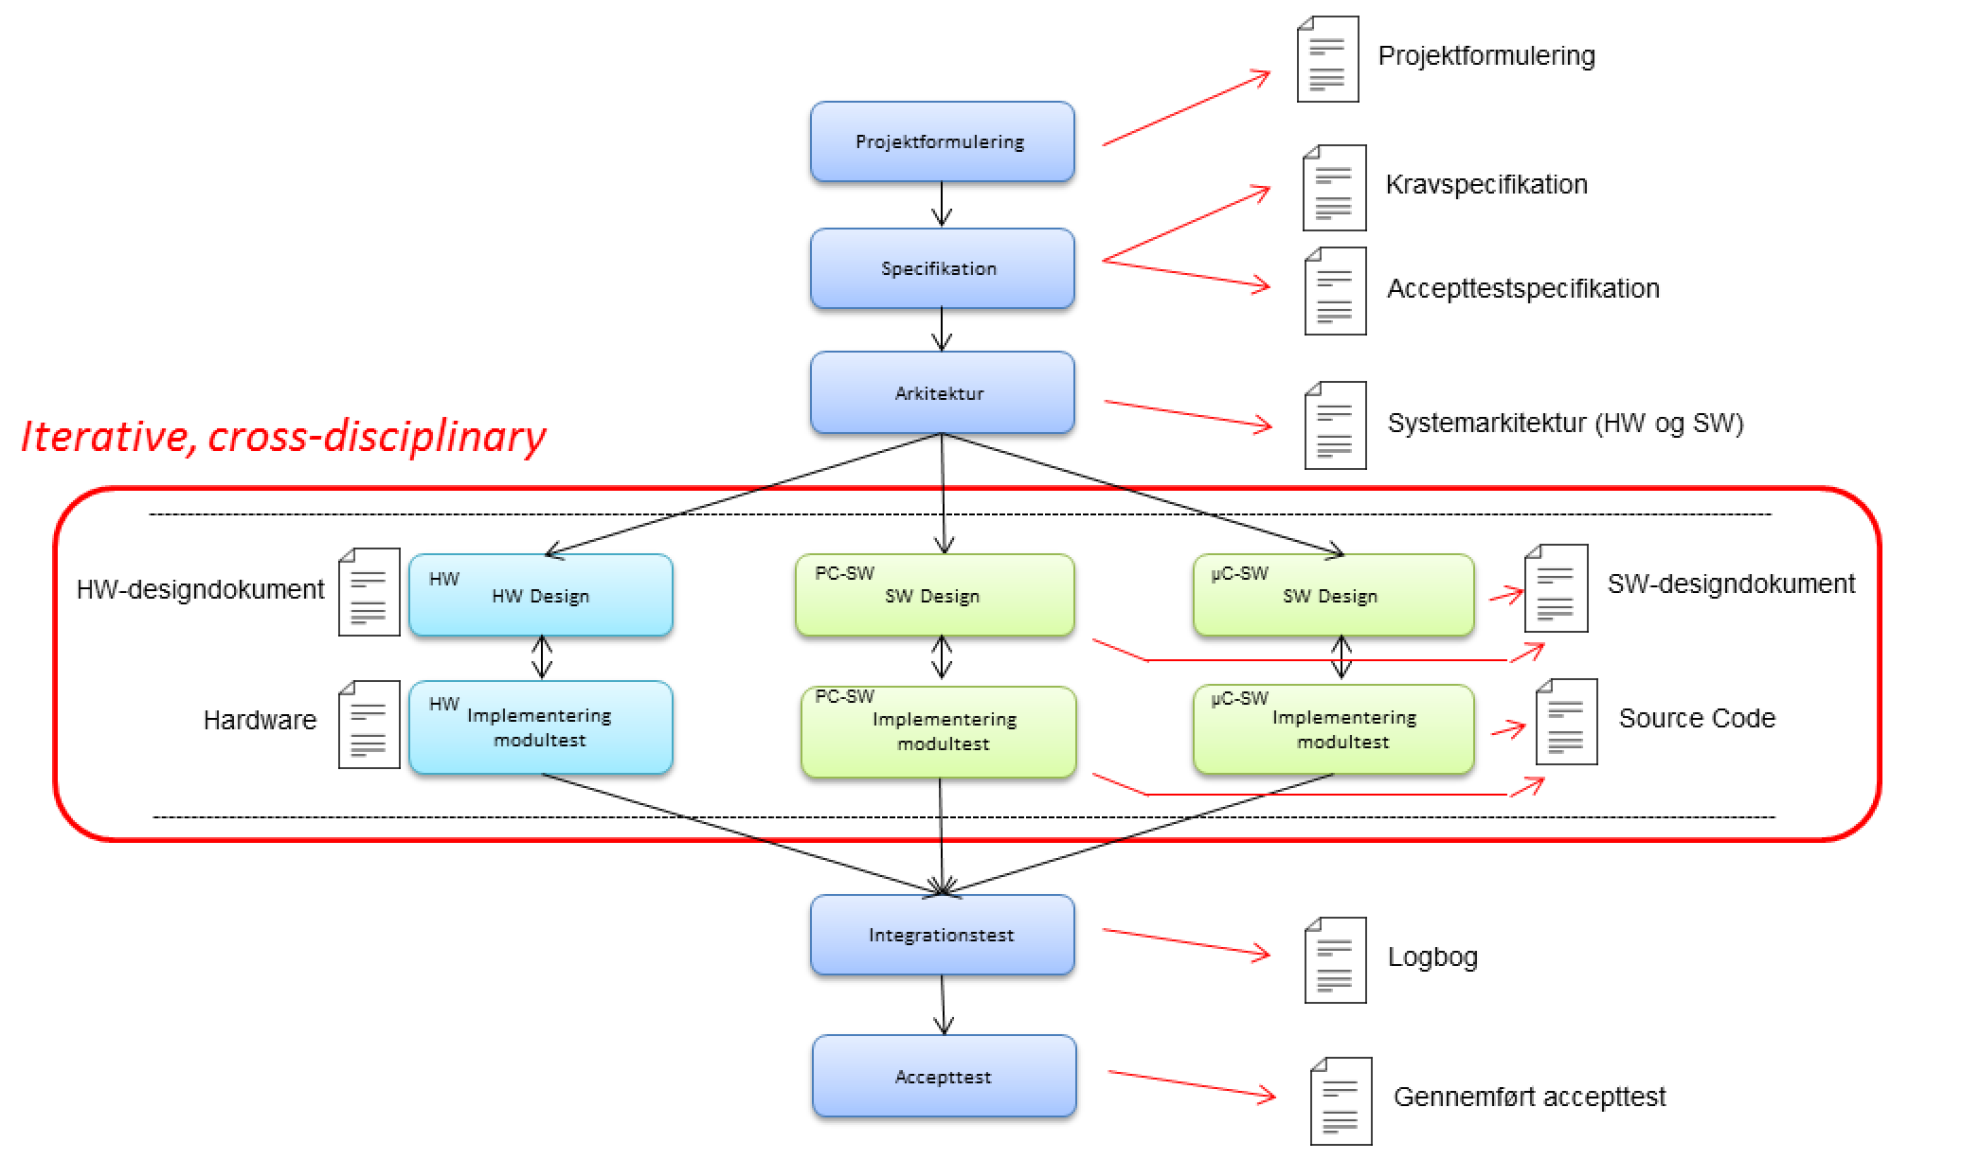
\includegraphics[max width=0.7\linewidth]{/tex/Billeder/ASEmodel.png}
	\caption{ASE model med fokus på iterativ proces~\cite{udviklingsproces}}
	\label{fig:ASE}
\end{figure} 
I begyndelsen blever produktet specificeret med krav, hvilket ikke har været iterativt, som det efterfølgende. Det skyldes at projektet er et oplæg fra Terma, som selv har specificeret kravene, og derfor har de været forholdsvis faste. Der har til dels stadig været krav, som senere i perioden er blevet lavet om efter samtaler mellem Terma og gruppen, men det er begrænset.

Til gengæld er det især design-, implementerings- og modultestfasen, der har fungeret iterativt. Det vil sige, at der forbedres på produktet i små bidder, eftersom der erfares mere og mere fra gang til gang. Ved hver iteration opstilles delmål forinden, som der opfyldes inden næste iteration påbegyndes. 
Til slut er der udarbejdet en accepttest, som kun er blevet udført én gang.

Det vil sige, at selvom der arbejdes iterativt, kan gennemførelsen stadig deles op i flere faser som vist i figur~\ref{fig:Iterative} 
\begin{figure}[H]
	\center
	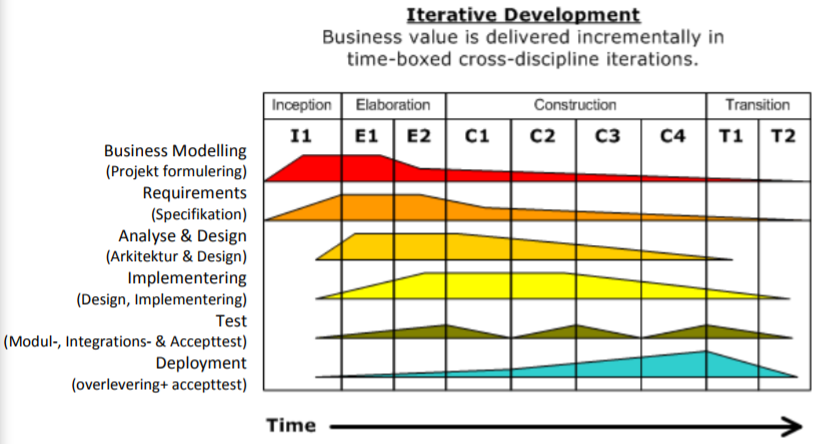
\includegraphics[max width=0.7\linewidth]{/tex/Billeder/Iterative.png}
	\caption{Udviklingsfaser og iterationer~\cite{udviklingsproces}}
	\label{fig:Iterative}
\end{figure} 
Her ses det hvordan design-, implementering- og testfaerne ligger oveni hinanden, mens specificeringen og afsluttende accepttest osv. er i højsædet i hhv. begyndelsen og slutningen.


Til at implementere udviklingsmodellen er det nødvendigt med et projektstyringsværktøj. Her faldt valget på scrum~\cite{Scrum}, da der er god erfaring med dette fra tidligere semesterprojekter. Scrum er henvendt til projektstyring og kan bruges i agile udviklingsprocesser. En del af Scrum går ud på at dele gruppens medlemmer op i mindre grupper med grupperoller. Denne del har ikke givet mening her, med en gruppe på 2. 
Til gengæld optimerer Scrum processen ved at reflektere over processen løbende og produktet deles op i mange små opgaver (backlog items). Opdeling og uddelegering af disse backlog items er for dette projekt gjort på et task board. Et øjebliksbillede af taskboardet kan ses på figur~\ref{fig:Taskboard} 
\begin{figure}[H]
	\center
	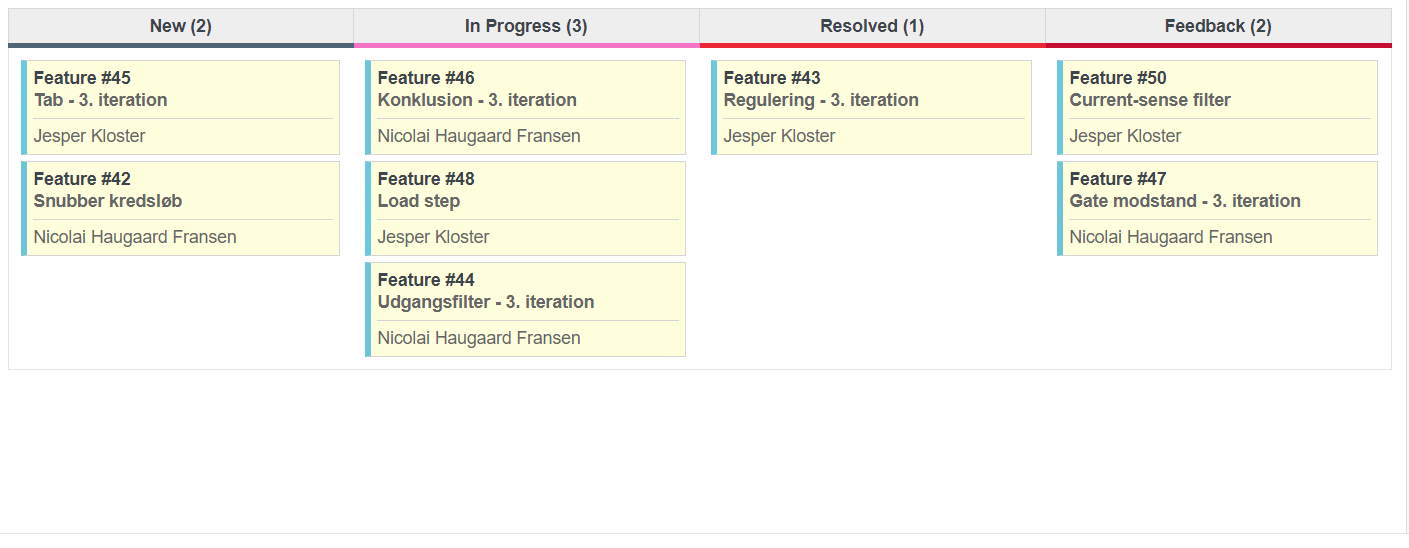
\includegraphics[max width=1\linewidth]{/tex/Billeder/Scrumtask.png}
	\caption{Scrum taskboard}
	\label{fig:Taskboard}
\end{figure} 
Overordnet set er taskboardsne yderligere delt ind i iterationerne. Her kigges på design-, implementering- og designfasens 3. iteration og dets backlog items, som på boardet kaldes features. De yderligere iterationer der er lavet i projektet er opstillet herunder:

\begin{itemize}
\item Specificering
\item Kravspecifikation
\item Systemarkitektur
\item Design, implementering og test 1. iteration
\item Design, implementering og test 2. iteration
\item Design, implementering og test 3. iteration
\item Accepttest
\item Dokumentation
\item Rapport
\end{itemize}

De enkelte iterationer har hver især gennemgået førnævnte iterative proces. Dog er design, implementering og test kaldt forskellige iterationer, for at bevare overblikket over ændringerne. Det ses på taskboardet hvordan de forskellige features begynder i "new". Derefter tager et medlem den feature man er i gang med, og flytter den til "in progress". Når featuren er færdig flyttes den til "feedback" Her bliver den rettet til af en anden fra gruppen, som efterfølgende flytter den til "resolved". Her kigges ændringer igennem af den oprindelige indehaver af featuren og til sidst flyttes featuren til "closed" og vises ikke på boardet mere. 
iteration er vurderet færdig, når alle features på taskboardet er flyttet til closed.
	\chapter{Projektledelse}
Som tidligere nævnt er der benyttet Scrum i projektet, men ikke projektledelses-delen af det. Det vil sige, at roller som Product Owner, Scrum Master osv. ikke har været på en bestemt person, men istedet været delt imellem gruppen. Det har været meget naturligt at gøre, med to medlemmer i gruppen. Det giver en flad struktur, hvor begge medlemmer har haft lige meget at sige og bestemt lige meget.  
	\chapter{Arbejdsfordeling}
Arbejdsfordelingen i forbindelse med produktets udvikling har været en blanding imellem, at kunne anvende forhåndsviden, og udfordre os selv ved at arbejde i ukendte områder. Der er startet op med en solid baggrundsviden fra faget "Effektelektronik", som gav kendskab til forskellige converter typer, så der forinden var et teoretisk grundlag at arbejde ud fra. Til gengæld har det vist sig, at udarbejdning af en converter i praksis bød på mange ting, som på forhånd var ukendt stof for gruppen.  

Det har givet en god mellemvej mellem kendte og ukendte ting, hvor en masse nyt stof er erfaret undervejs, og hvor gruppen ikke alt for ofte har befundet sig på bar bund, men har kunnet drage paralleller til undervisningen.

Til selve fordelingen af arbejdsopgaver, er der brugt Scrum taskboard, som nævnt i sektion~\ref{udvikling}. Det har fungeret ganske godt, da det selv med en gruppe på to, er vigtigt at kunne holde et godt overblik. Samtidig kan man altid sikre sig, at der ikke er to i gang med den samme opgave, ved at kigge på taskboardet. Det er også en god måde, at holde øje med at alle medlemmer tager nok opgaver, og at det ikke kun er en enkelts navn, der står på dem alle. Igen har det ikke været et problem i dette projekt, hvor opgave fordelingen har været helt lige.     
	\chapter{Planlægning}
For at planlægge det tidsmæssige aspekt af projektet, er tidsplanen benyttet, hvilken er vedlagt i bilagsmappen. Den er delt op i de forskellige iterationer, som processen har været opdelt i. Iterationerne er listet op i sektion~\ref{udvikling}. I tidsplanen er der fra første uge forsøgt, at opskrive planlagte tidspunkter for begyndelse og færdiggørelse af hver enkelt iteration. 
	\chapter{Projektadministration}
Projektadministreringen er noget af det første der blev fastlagt i projektet, da det fremskønner processen og sørger for der er enighed om hvordan tingene udføres og sættes op. 

Konfigurationsstyringen er gjort ved brug af Githubs repository~\cite{Github}. Det er et program, der kan bruges til deling af dokumenter og versionshistorik af disse. Yderligere er rapport, dokumentation og procesbeskrivelse skrevet i programmet LaTeX~\cite{Latex}. Kombinationen mellem LaTeX og Github gør det nemt, at merge ændringer i dokumenterne. Det giver mulighed for, at redigere eller skrive i samme dokument, uden det skaber problemer. Samtlige dokumenter og bilag, der er vedlagt, har været administreret over Github.  

Den interne kommunikation i gruppen er foregået over facebook. Her er der kommunikeret omkring mødetider, spørgsmål og generelt delt information. Dokumenter osv. er som beskrevet ikke en del af facebookgruppen, men delt ved hjælp af Github.
Den eksterne kommunikation med både vejleder og kontaktpersoner fra Terma er foregået over mail. 
	\chapter{Møder}
Der har været afholdt tre forskellige slags møder i løbet af processen. Det indebærer interne gruppemøder, vejledermøde med Arne Justesen og eksterne møder med kontaktpersonerne fra Terma, Johnny Laursen og Hans Jensen.  

De interne møder har været brugt hver dag i form af det daglige scrum møde, også kaldet "stå op møde". Her begyndes dagen med at hvert medlem reflektere over gårsdagens arbejde, og hvad der skal indtil næste møde. Eventuelle problemer med en given opgave opgives her, og findes der ikke en hurtig løsning, gås der i dybden med det efter mødet. 

Langt hen af vejen har der været afholdt vejledermøde en gang i ugen. Her har der forinden været sendt en dagsorden til vejleder, der beskriver hvad mødet vil handle om, og måske indeholde nogle dokumenter der skal gennemlæses inden mødet. 

Møderne har indeholdt en gennemgang af fremskridt den seneste uge, og planen for den næste uge. Derudover har der været uddybende snakke omkring tekniske og rapportmæssige problemer, der opstod undervejs. Der har ikke været deciderede sprint retrospectives, da der har været afholdt møder i hver uge, og sprintsne har varet mere end det. De ugentlige møder minder dog meget om det, da der har været snak om den forgangne uge ved hvert møde og udbyttet af det, ligesom ved retrospectives. 

Til hvert møde har der været brugt en referent, der har haft til opgave at fange og skrive essensen af samtalerne. Derudover har det andet gruppemedlem fungeret som mødeleder, og har haft til ansvar at lede mødet med henblik på dagsordenen. På den måde sikres det både, at mødet gennemgår alle de tænkte punkter og det hele bliver dokumenteret. Mødeleder og referent er gået på skift fra møde til møde.    

I en måned midtvejs i projektet har projektets vejleder været sygemeldt, og Emir Pasic har været standin i den periode. Da hans kendskab til selve stoffet er begrænset, var det mere den rapportmæssige del han kunne bidrage til. Da projektet i denne periode var i design-, implementerings- og testfasen, blev det meste tid brugt på Terma, og derfor blev udbyttet af standin-vejlederen begrænset.      

Der har været afholdt møder med kontaktpersonerne fra Terma næsten hver uge. Igen har der været sendt information til kontaktpersonerne om, hvad der ønskes at opnå til møderne. Til disse møder har der været rigtig god mulighed for, at diskutere de faglige problemer, der er opstået undervejs. Igen har der været brugt en mødeleder og en referent, som også her er gået på skift.  
I design-, implementerings- og testfasen har der dagligt været faglige diskussioner. Det har været produktivt, at kunne få svar på et problem med det samme, i stedet for at skulle vente på det næste ugentlige møde. Mødereferater kan findes i den vedlagte bilagsmappe. 
	
	%\include{<sti/filnavn.tex>}
	
	%%% Foreløbig disposition %%%
	% Introduktion
	%% Projektformulering/Motivation?
	%% Systembeskrivelse
	%% Systembetragtning
	% Kravspecifikation
	% Systemarkitektur
	%% HW
	%% SW
	% Accepttest
	
	\printbibliography[title={Litteraturliste}]
	
\end{titlingpage}
\end{document}